\documentclass[11pt]{article}
\usepackage[margin=0.8in]{geometry}
\usepackage{amsmath,amssymb,amsthm,booktabs,graphicx,xcolor,hyperref,microtype}
\hypersetup{colorlinks=true,urlcolor=blue,linkcolor=blue,citecolor=blue}
\emergencystretch=2em
\newtheorem{theorem}{Theorem}
\newcommand{\R}{\mathbb R}
\title{When Plans Change,\\How Far Can a Robot Stray?\\[4pt]
\large A checked tracking bound for an axis with uncertain lag}
\author{Mike\\\small Local research note; author details and affiliation pending}
\date{17 October 2026}
\begin{document}
\maketitle
\begin{abstract}
A smooth plan is a statement about desired motion. It does not bound the motion of the machine that follows it. We connect constant-jerk reference segments to a scalar axis with uncertain, time-varying actuator lag. A Lean proof derives the error dynamics from the plant and preserves an error tube across any finite matched sequence of replans. The same proof gives travel margins and input bounds. A proved change of time scale makes the plant assumptions explicit. We compare three feedforward choices and expose a tradeoff: the choice that tightens this uniform certificate need not give the best short-time response. The result is a reproducible formal case study. It is not a new general robot controller or evidence of hardware safety.
\end{abstract}

\section{A concrete question}
An axis follows a sequence of plans. The next plan can change while the axis is moving. Each new reference starts at the old reference's position, velocity, and acceleration. The physical axis keeps its own state. We ask how much space must remain between the planned path and a travel limit.

\begin{figure}[htbp]
\centering
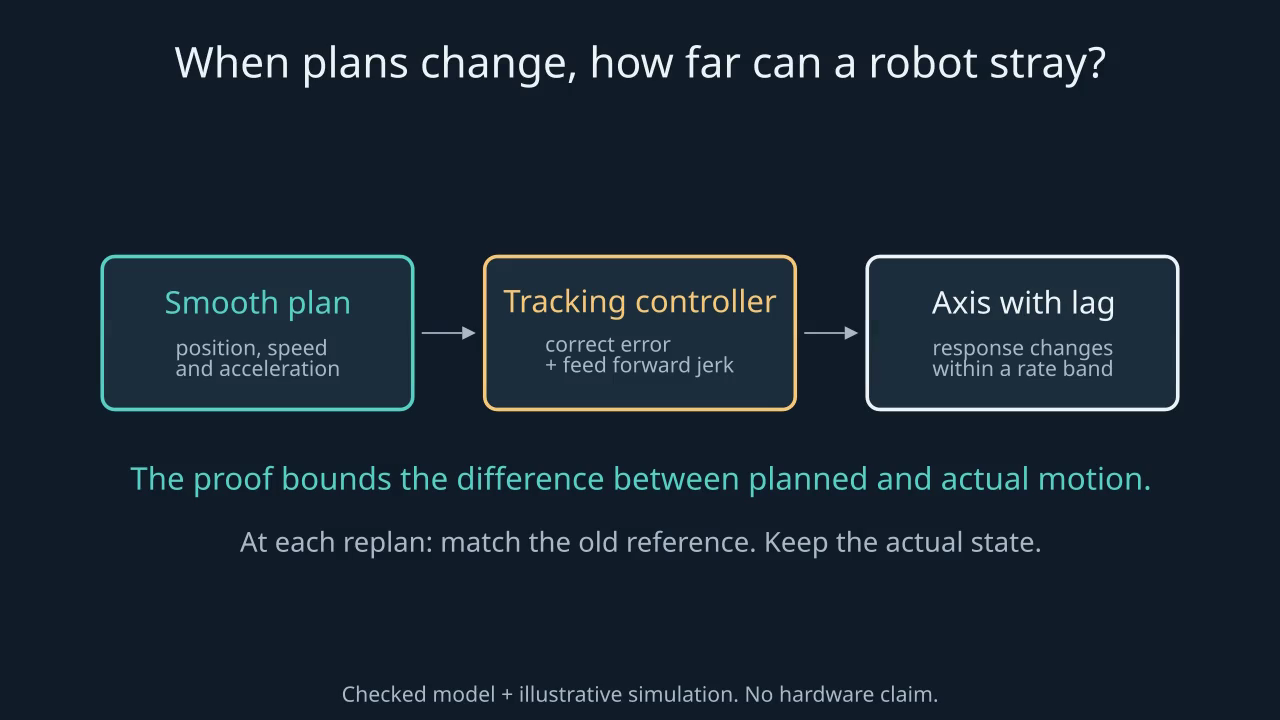
\includegraphics[width=\textwidth]{images/model.png}
\caption{Frame from the accompanying Manim explanation. The reference and the actual axis are different state trajectories. A matched replan preserves the reference state while the physical axis continues from its own state.}
\end{figure}

The model is one axis on a rail. Its state is position $x$, velocity $v$, and acceleration $a$:
\begin{equation}\label{eq:plant}
 \dot x=v,\qquad \dot v=a,\qquad \dot a=r(t)(u+w-a).
\end{equation}
The actuator rate obeys $8\sigma\le r(t)\le12\sigma$, where $\sigma>0$.
The additive target error satisfies $|w(t)|\le W$. On each open segment, a reference $(q,v_q,a_q)$ obeys
$\dot q=v_q$, $\dot v_q=a_q$, and $\dot a_q=j$, with $|j|\le J$.
Constant-jerk segments are a checked instance.

Let $e_x=x-q$, $e_v=v-v_q$, and $e_a=a-a_q$. Use the controller
\begin{equation}\label{eq:control}
 u=a_q-8\sigma^2 e_x-6\sigma e_v-\tfrac12 e_a
       +\frac{5}{48\sigma}j.
\end{equation}
The coefficients carry the units required by the displayed physical model.
Larger $\sigma$ requires a faster \emph{actual} actuator. Increasing gains alone does not establish the new rate band.

\section{The checked claim}
Define the three error coordinates
\[
 z_0=e_x,\qquad z_1=e_x+\frac{e_v}{4\sigma},\qquad
 z_2=e_x+\frac{e_v}{2\sigma}+\frac{e_a}{16\sigma^2}.
\]
They describe a tilted box in the physical error state.

\begin{theorem}[Tracking through finite replans]\label{thm:track}
Let $R\ge0$, $\sigma>0$, and let each segment have nonnegative finite duration.
Assume the physical state and reference are continuous on each closed segment.
Assume their stated differential equations hold on each open segment.
Assume the rate, disturbance, and reference jerk bounds hold throughout each segment.
If
\[
 W+\frac{J}{48\sigma}\le2\sigma^2R
 \quad\hbox{and}\quad |z_i(0)|\le R\quad(i=0,1,2),
\]
then $|z_i(t)|\le R$ throughout that segment.
The same cube is preserved through any finite sequence whose actual states and reference states match separately at each boundary.
In particular,
\[
 |x-q|\le R,\qquad |v-v_q|\le8\sigma R,\qquad
 |a-a_q|\le64\sigma^2R.
\]
\end{theorem}
There is no minimum dwell time in this finite composition theorem.
It makes no assertion about infinitely many switches in finite time.
It is conditional on the stated trajectories; it does not construct executions for arbitrary irregular inputs.

\paragraph{Why it works.}
Set normalized time $\tau=\sigma t$ and normalized error
$E=(e_x,e_v/\sigma,e_a/\sigma^2)$.
The chain rule gives the earlier robust holding model with rate $r/\sigma\in[8,12]$.
Its effective normalized disturbance is
\[
 \frac{1}{\sigma^2}\left[w+
       \left(\frac{5}{48\sigma}-\frac1r\right)j\right].
\]
The interval $1/(r/\sigma)\in[1/12,1/8]$ has center $5/48$ and radius $1/48$.
The budget above therefore gives the required disturbance bound $2R$.
The inherited invariant-cube theorem applies.
Matching both state triples at a switch preserves their difference.
Induction then proves the finite sequence result.
Lean checks the plant reduction, time change, cube reuse, and finite composition.

\paragraph{Travel and actuator margins.}
If $q(t)\in[L+R,U-R]$, then $x(t)\in[L,U]$.
If $|a_q|\le A$, then
\[
 |u+w|\le A+24\sigma^2R+\frac{5J}{48\sigma}+W.
\]
The existing Bernstein control-point test checks bounds on a whole constant-jerk reference segment.
The unscaled admitted-segment theorem combines that test with the tracking result.
A failed sufficient test does not prove unsafe motion.

\section{A comparison with two answers}
Keep the same plant, feedback gains, and reference. Change only jerk feedforward.
Acceleration feedforward $a_q$ remains in all three controllers.
For $\sigma=1$, the choices are:
\begin{center}
\begin{tabular}{lcc}
\toprule
Jerk coefficient $\kappa$ & $\max_r|\kappa-1/r|$ & $\max_r|r\kappa-1|$\\
\midrule
$0$ & $1/8$ & $1$\\
$1/10$ & $1/40$ & $1/5$\\
$5/48$ & $1/48$ & $1/4$\\
\bottomrule
\end{tabular}
\end{center}
The first metric controls the disturbance budget used by this cube.
Its minimax choice is $5/48$.
The second metric controls initial acceleration-error growth from zero tracking error when $w=0$.
Its minimax choice is $1/10$.
Lean checks both minimax inequalities.
For general $\sigma$, divide the three coefficients and the first metric by $\sigma$.

The reciprocal midpoint reduces the worst jerk contribution to this certificate by a factor of six compared with omitting jerk feedforward.
It does not establish a sixfold reduction in observed error.
Nor is the resulting sufficient radius the smallest possible tracking bound.
For constant rate and constant forcing, a steady error can be much smaller.

\begin{figure}[htbp]
\centering
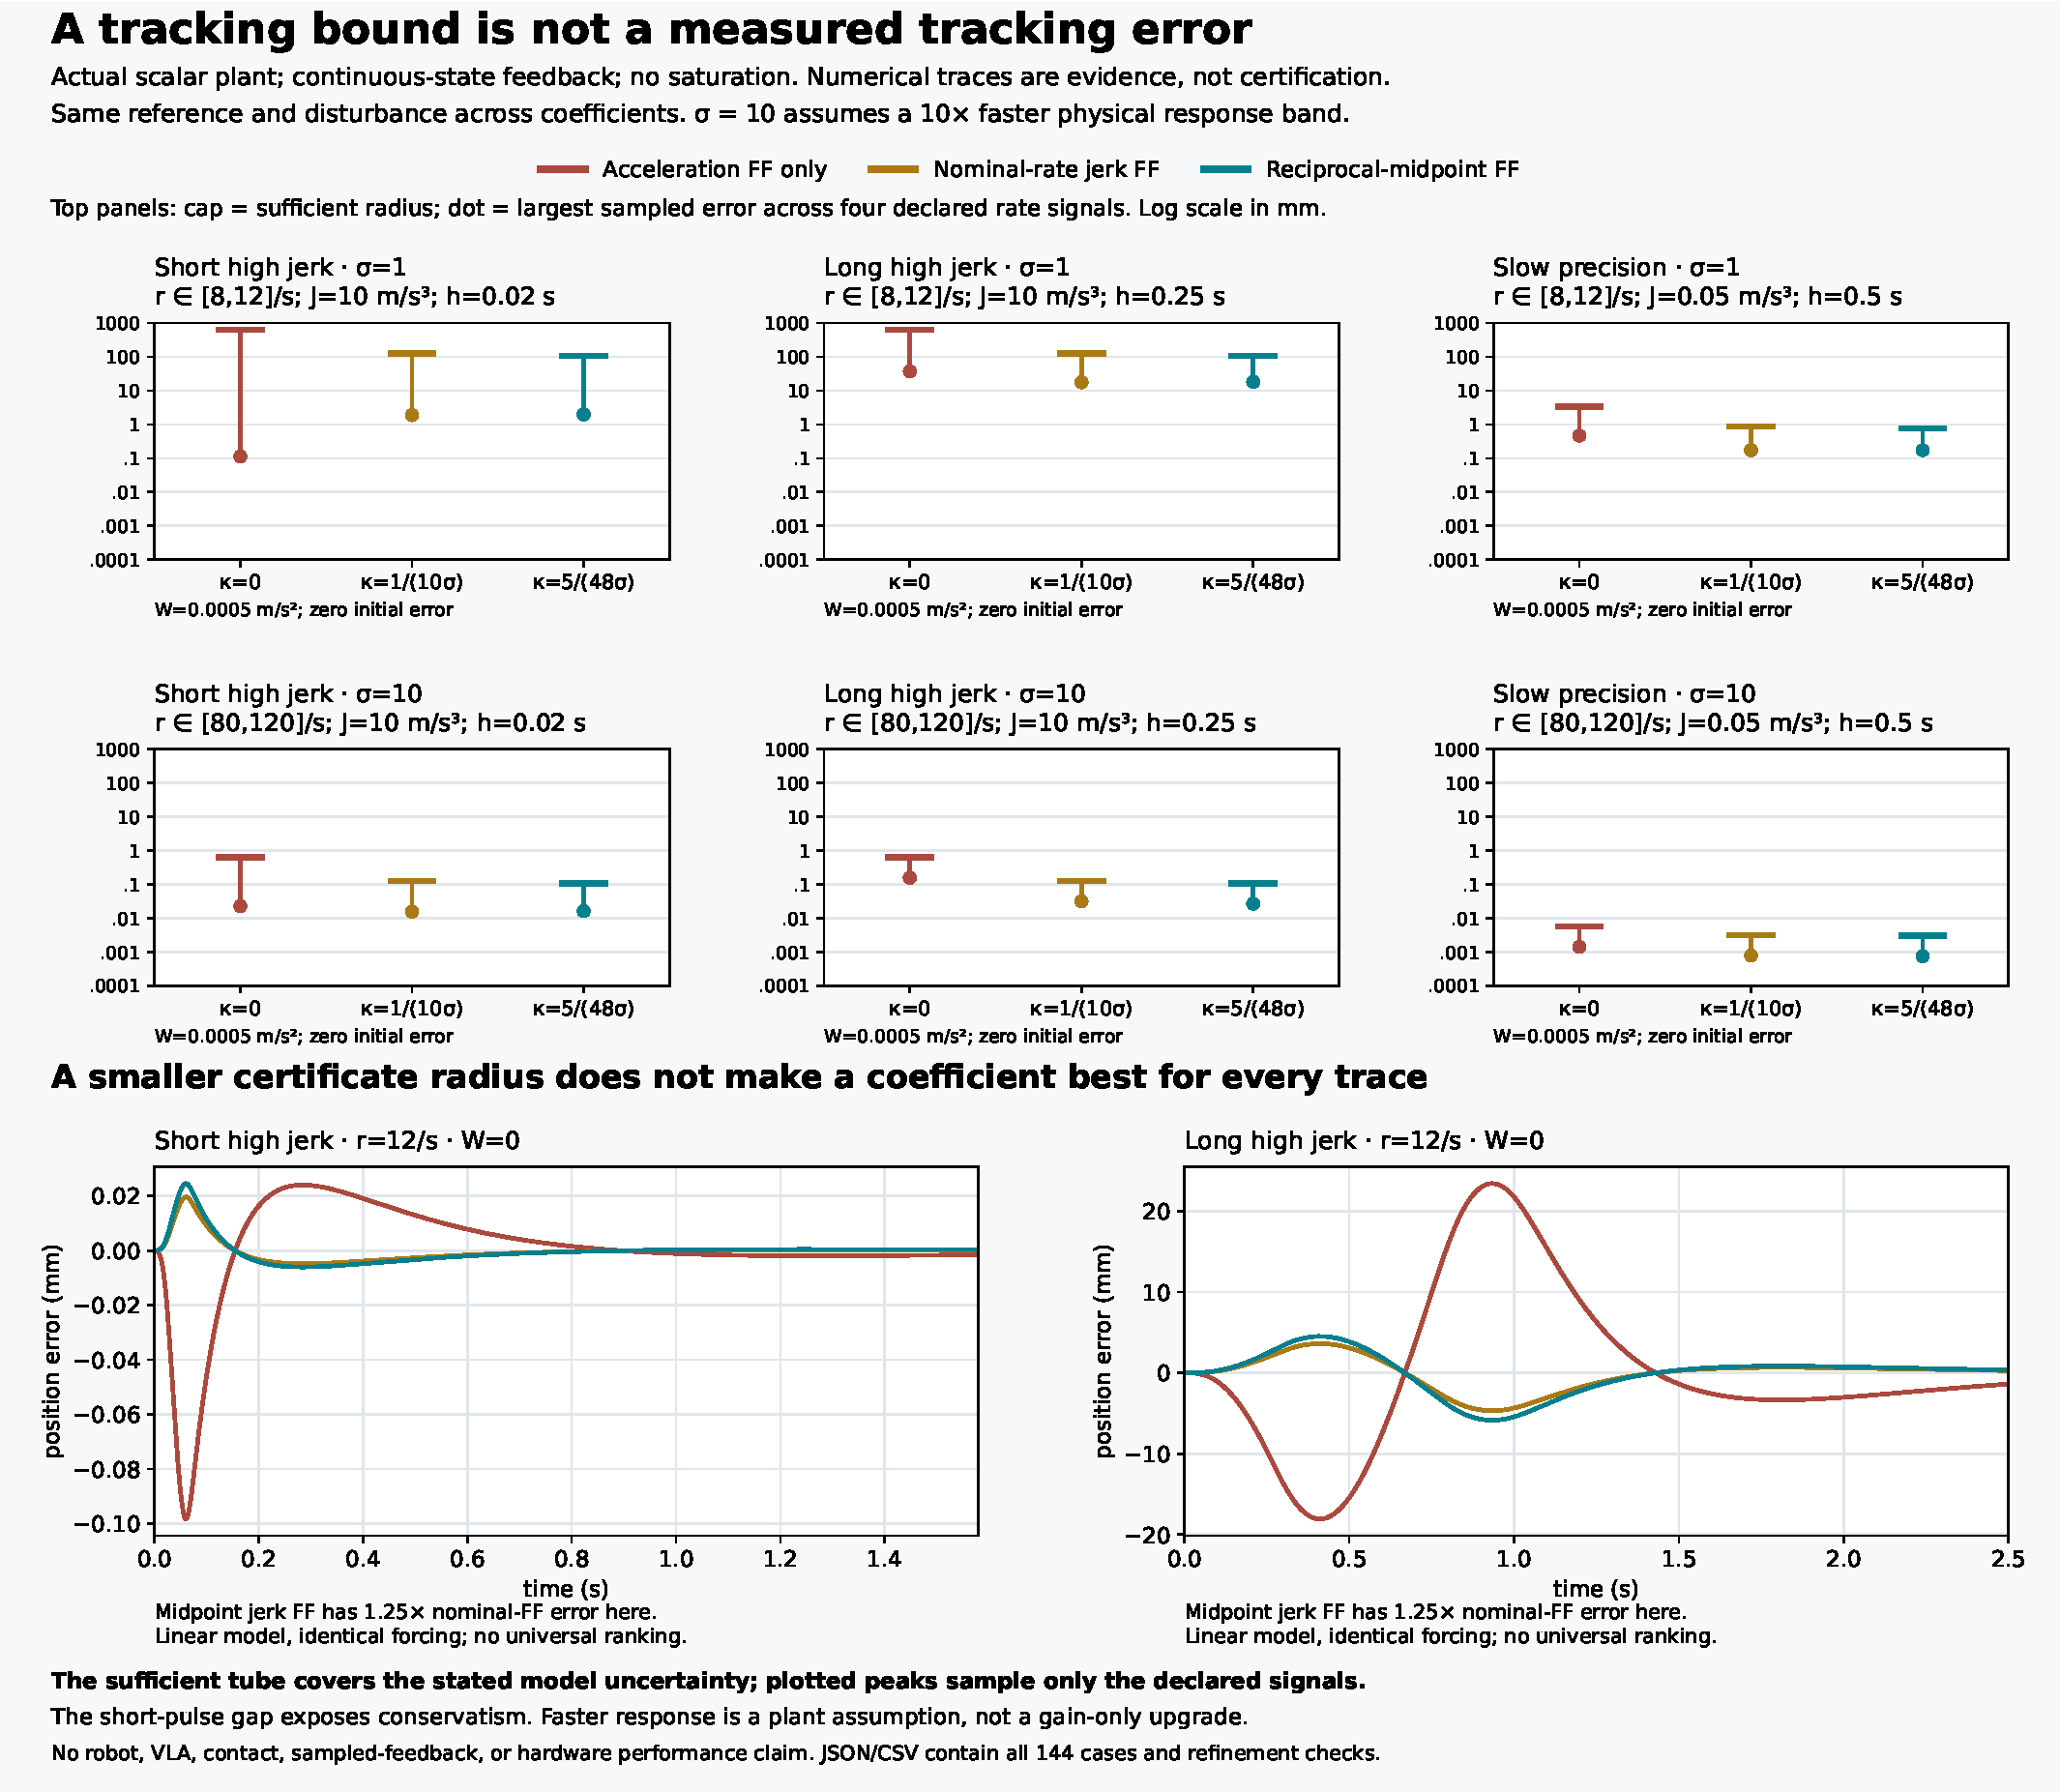
\includegraphics[width=\textwidth]{images/comparison.pdf}
\caption{Reproducible numerical comparison. Solver traces illustrate selected inputs; they do not replace the interval theorem. Each scaled case uses the corresponding physical actuator rate band.}
\end{figure}

\paragraph{What the numerical comparison found.}
The experiment covers 144 cases with three reference profiles, two physical rate scales, four rate signals, two disturbance budgets, and three feedforward choices. Every case is integrated twice. The largest sampled position difference between the coarse and refined runs is $1.42\times10^{-10}\,\mathrm m$.
This tests numerical consistency; it does not prove a continuous-time envelope.

For $W=0.0005\,\mathrm{m/s^2}$, the table reports the largest sampled position error among the four tested rate signals. All errors include the four-second hold after the motion.
The slow-axis case moves the reference by only $0.16\,\mathrm{mm}$.
The fast-axis case moves it by $312.5\,\mathrm{mm}$.
\begin{center}
\begin{tabular}{lrr}
\toprule
Jerk coefficient & Slow axis ($\sigma=1$) & Fast axis ($\sigma=10$)\\
 & peak error (mm) & peak error (mm)\\
\midrule
$0$ & 0.11245 & 0.15642\\
$1/(10\sigma)$ & 1.88368 & 0.03176\\
$5/(48\sigma)$ & 1.96018 & 0.02671\\
\bottomrule
\end{tabular}
\end{center}
The hand-chosen varying rate can bias the jerk feedforward over a short signed sequence. It is a bounded stress signal, not a proved worst case. Its poor slow-axis result rules out a universal performance claim. The sufficient slow-axis radii are also much wider than these measured errors. The numerical and proof questions must stay separate.

\paragraph{An illustrative specification.}
Take $\sigma=10$, so the rate must stay in $[80,120]\,\mathrm{s}^{-1}$.
Let $W=0.01\,\mathrm{m/s^2}$, $J=10\,\mathrm{m/s^3}$, and $R=0.2\,\mathrm{mm}$.
Then the budget is $0.030833\ldots\le0.04$ in acceleration units.
If the initial cube fits and the physical assumptions hold, the position error stays within $0.2\,\mathrm{mm}$.
The corresponding velocity and acceleration error margins are $0.016\,\mathrm{m/s}$ and $1.28\,\mathrm{m/s^2}$.
The effective input margin above $A$ is $0.594166\ldots\,\mathrm{m/s^2}$.
These are example specifications, not measured robot performance.

\section{What the result does and does not settle}
The proof connects a smooth reference to an uncertain physical axis model.
It does not establish an end-effector bound for a coupled arm, contact task, flexible mechanism, or VLA policy.
It uses continuous access to the physical state.
Sensor error, sample age, delay, and command hold must be derived into a valid $W$ before deployment.
Input clipping must also be covered; a clipped plant cannot silently use the unclipped equation.

A reference jerk bound is not an identical bound on actual jerk.
At zero error and $w=0$, the acceleration derivative is $r\kappa j$.
For $r=12$ and $\kappa=5/48$, that factor is $1.25$.
The unscaled Lean theorem instead bounds actual jerk on each open segment by
$12(56R+|\kappa|J+W)$.
A derivative need not exist at a jerk switch.
Bounded tracking does not guarantee target completion, a feasible future plan, or a safe stop from every intermediate state.

\paragraph{Relation to prior work.}
Higher-order trajectory generation and feedforward are established~\cite{lambrechts}.
Ruckig provides a richer real-time jerk-limited trajectory generator~\cite{ruckig}.
FaSTrack already connects planning models to tracking models through an error bound~\cite{fastrack}.
RTD addresses repeated planning with reachable sets and persistent feasibility~\cite{rtd}.
VeriPhy spans proof-to-executable controller verification~\cite{veriphy}.
Our narrower contribution is a small explicit Lean proof chain for this uncertain axis, with stated margins and a comparison that distinguishes two feedforward objectives.
These sources do not establish novelty of our artifact.

\paragraph{Reproduction and completion boundary.}
The source is in \path{research/adjacent-controls/tracking-replans/}.
Run \texttt{python3 verify.py} there with the workspace's pinned Lean setup.
The report records source hashes, a fresh build of local dependencies, axiom closures, separate kernel replays, and rejection of two false mutations.
It reuses pinned compiled LeanControls and Mathlib dependencies.
Run the documented numerical command separately for the comparison.
The theorem check validates the formal implication. It does not validate the physical assumptions.

The final local verification passed for all 34 target statements, including both separate kernel replays and both deliberately false mutations. This completes the stated local technical artifact.
A submission still needs a precise venue contribution, an implementation bridge, and stronger independent review.
An identified hardware axis or a calibrated simulation would make the next study more useful. This deterministic motion bound is not a PL d or PL e reliability assessment.
AI tools assisted proof construction, experiments, writing, and critique. Their agreement is not peer review.

\begin{thebibliography}{9}\small
\bibitem{lambrechts} P. Lambrechts, M. Boerlage, and M. Steinbuch.
Trajectory planning and feedforward design for high performance motion systems.
ACC, 2004.
\href{https://skoge.folk.ntnu.no/prost/proceedings/acc04/Papers/0827_FrM03.2.pdf}{Primary paper}.
\bibitem{ruckig} L. Berscheid and T. Kr\"oger.
Jerk-limited real-time trajectory generation with arbitrary target states.
RSS, 2021.
\href{https://roboticsproceedings.org/rss17/p015.html}{Paper record}.
\bibitem{fastrack} M. Chen et al.
FaSTrack: a modular framework for real-time motion planning and guaranteed safe tracking.
IEEE Transactions on Automatic Control, 2021.
\href{https://arxiv.org/abs/2102.07039v2}{arXiv:2102.07039v2}.
\bibitem{rtd} S. Kousik et al.
Bridging the gap between safety and real-time performance in receding-horizon trajectory design for mobile robots.
International Journal of Robotics Research, 2020.
\href{https://arxiv.org/abs/1809.06746v2}{arXiv:1809.06746v2}.
\bibitem{veriphy} R. Bohrer et al.
VeriPhy: verified controller executables from verified cyber-physical system models.
PLDI, 2018.
\href{https://doi.org/10.1145/3192366.3192406}{doi:10.1145/3192366.3192406}.
\end{thebibliography}
\end{document}